\dbname was built from videos from the YouTube channel CN Sordos, a news channel created in 2020 by deaf people and deaf people's relatives. The hosts use LSA to communicate the news. Subtitles in Spanish are provided by the authors. There are two main hosts in most of the videos. There are other regular hosts in charge of special sections like ecology or movies, but these appear much less often. Therefore, the great majority of the 103 signers present on the dataset are guests who appear once or twice for an interview or a specific piece of news. There is gender parity among the signers and videos contain different locations, backgrounds and lighting conditions.

\dbname was generated in two stages. In the first stage, we collected the videos and cropped them according to its subtitles. For each valid sentence in the subtitles of a video (annotations like "[background music]" were discarded), we cropped the corresponding video clip. This process resulted in 14,880 video segments. In the second stage, in those segments where there is more than one person, we inferred who is the signer with a certain score of confidence. Section \ref{subsec:signer_inference} describes how this inference was done. 

Finally, we also made available a visualization tool so that researchers can easily explore the dataset. The tool was developed using Fifty One \cite{moore2020fiftyone}, which provides useful features such as allowing to filter samples by label, video, playlist, or by the confidence score of the signer inference.

Full code for the development of this dataset, the analysis described below, and the start-up of the visualization tool can be found in the project's repository\footnote{\dbrepourl}.

\subsection{Statistics and analysis}\label{subsec:stats}

\dbname was built from 63 different videos of the CN Sordos Channel. We only used videos that had been annotated with subtitles by the authors (LSA experts). The videos resulted in 14,880 segments that span 21.78 hours of video. Each sample of the database contains a sentence taken from the subtitles provided and its respective video segment. The generated segments have a mean duration of 5.27 seconds and their labels a mean of 4.78 words per sample (Figure \ref{fig:clips_statistics}).

\begin{figure}
    \centering
    \begin{subfigure}[b]{0.38\textwidth}
        \centering
        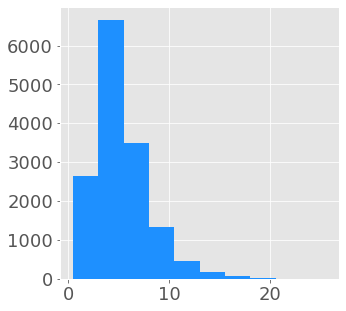
\includegraphics[width=\textwidth]{images/hist_times_per_vid.png}
        \caption{}
        \label{subfig:hist_times_per_vid}
    \end{subfigure}
    \hfill
    \begin{subfigure}[b]{0.38\textwidth}
        \centering
        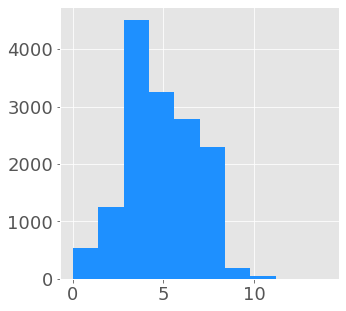
\includegraphics[width=\textwidth]{images/hist_words_per_vid.png}
        \caption{}
        \label{subfig:hist_words_per_vid}
    \end{subfigure}
    \hfill
    \caption{Histograms of segments duration (a) and amount of words per sentence (b).}
    \label{fig:clips_statistics}
\end{figure}

As shown in Table \ref{tab:bd_comparison}, a peculiarity of the dataset is the significant proportion of unique sentences (\(\sim95\%\)) and the proportion of unique words with respect to the vocabulary size (\(\sim50\%\)) (\ref{subfig:hist_word_freq}). Therefore, we consider the dataset to be highly challenging for a SLT model. 

A common preprocessing step in the natural language processing field consist on removing sentences with words that appear very few times in the dataset so they do not add noise to the training process. Histograms of word frequencies after removing samples with singletons and words with frequencies lower than 5 are shown in figures \ref{subfig:hist_words_freq_no_sing} and  \ref{subfig:hist_words_freq_no_lt5}, respectively. After removing the corresponding subset of labels, the histograms do not show such a heavy left tail, despite the fact that other words now appear with a lower frequency than before.

\begin{figure}
    \centering
    \begin{subfigure}[b]{0.32\textwidth}
        \centering
        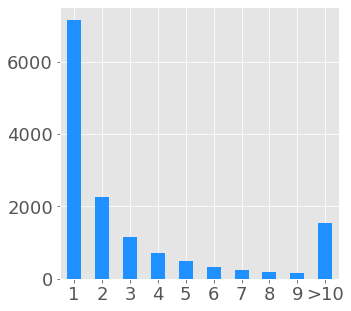
\includegraphics[width=\textwidth]{images/hist_words_freq_grouped_gt10.png}
        \caption{}
        \label{subfig:hist_word_freq}
    \end{subfigure}
    \hfill
    \begin{subfigure}[b]{0.32\textwidth}
        \centering
        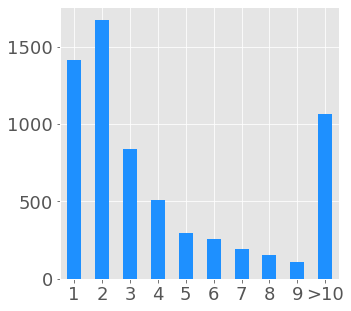
\includegraphics[width=\textwidth]{images/hist_words_freq_no_sing_grouped_gt10.png}
        \caption{}
        \label{subfig:hist_words_freq_no_sing}
    \end{subfigure}
    \hfill
    \begin{subfigure}[b]{0.32\textwidth}
        \centering
        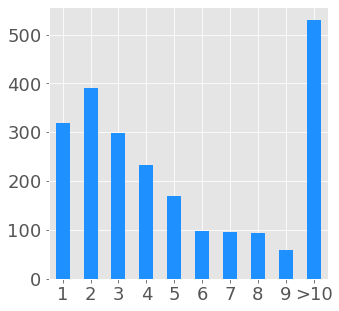
\includegraphics[width=\textwidth]{images/hist_words_freq_no_lt5_grouped_gt10.png}
        \caption{}
        \label{subfig:hist_words_freq_no_lt5}
    \end{subfigure}
    \caption{Histograms of word frequency over the whole dataset (a), after removing samples with singletons (b) and and after removing samples with words with frequency lower than 5 (c).}
    \label{fig:words_statistics}
\end{figure}

Finally, figures \ref{subfig:bar_30_most_common_words_freq} and \ref{subfig:bar_30_most_common_trigrams_freq} show the 30 most commons words and trigrams respectively. As many of the most common words correspond to articles or connectors we believe the trigrams can provide a more representative visualization of the dataset content. Additionally, we expect traditional models without special training schemes to be able to learn these common trigrams.

\begin{figure}
    \centering
    \begin{subfigure}[b]{0.4025\textwidth}
        \centering
        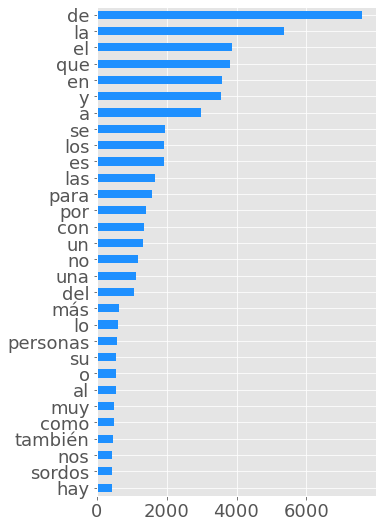
\includegraphics[width=\textwidth]{images/bar_30_most_common_words_freq.png}
        \caption{}
        \label{subfig:bar_30_most_common_words_freq}
    \end{subfigure}
    \hfill
    \begin{subfigure}[b]{0.57\textwidth}
        \centering
        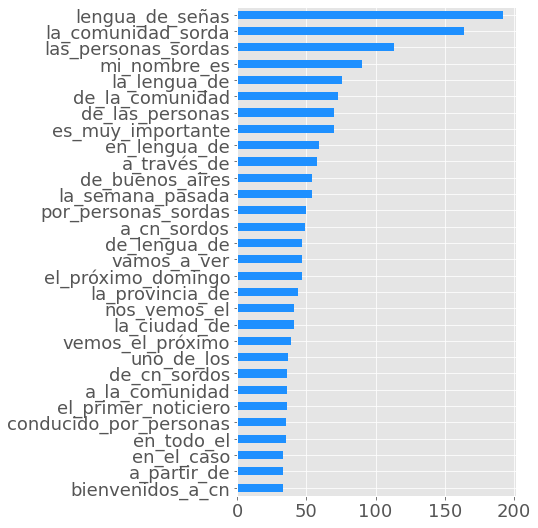
\includegraphics[width=\textwidth]{images/bar_30_most_common_trigrams_freq.png}
        \caption{}
        \label{subfig:bar_30_most_common_trigrams_freq}
    \end{subfigure}
    \hfill
    \caption{Most common words (a) and trigrams (b) in the dataset}
    \label{fig:most_common_words_trigrams}
\end{figure}

\subsection{Default Train-Test sets}\label{subsec:train_test_split}

Alongside the dataset, we provide two versions of the train and test sets: a full version and a reduced version. We made the reduced version by excluding labels that contain words with frequency lower than 5. This version is expected to be easier for a SLT model to learn. In both versions we used 80\% of the samples for training and 20\% for testing. Samples with a signer-confidence score lower than 0.5 were discarded (section \ref{subsec:signer_inference}).

Also, as videos labels are subtitles instead of classes, traditional stratified Train-Test splits cannot be performed. Since samples from the same video are expected to share topics and therefore vocabulary, both train and test sets were generated so that segments from the same video are included in both.

\begin{table}
\caption{Comparison between the two versions of the train-test sets.}
\label{tab:train_test_comparison}
\begin{center}
    \begin{tabular}{ |p{4cm}|c|c c|c c| }
        \hline
        & \dbname & \multicolumn{2}{|c|}{Full version} & \multicolumn{2}{|c|}{Reduced version}\\ 
        & & Train & Test & Train & Test \\
        \hline
        %signers & 103 & X & X & X & X\\
        %duration [h] & 21.78 & 17.49 & 4.29 & 15.85 & 3.89\\
        \# sentences & 14,880 & 11,065 & 2735 & 3767 & 910\\
        \% unique sentences & 95.79\% & 96.64\% & 92.78\% & 96.88\% & 98.35\%\\
        \hline
        vocab. size & 14,239 & 12,385 & 5546 & 2694 & 1579\\
        \% singletons & 50.21\% & 52.01\% & 61.9\% & 23.2\% & 48.83\%\\
        \% sentences with singletons & 34.97\% & 40.98\% & 67.97\% & 14.36\% & 54.29\%\\
        \% sentences with words not in train vocabulary & - & - & 59.2\% & - & 84.5\%\\
        \hline
    \end{tabular}
\end{center}
\end{table}

Table \ref{tab:train_test_comparison} shows a comparison between the different versions. As it can be seen, there is no significant difference between them in terms of percentage of unique sentences, but there is in terms of percentage of singletons. While in the full version around 50\% of the training vocabulary are singletons, only 23\% of the train vocabulary of the reduced version are. Furthermore, while 40\% of the labels on the full version train train contain singletons, only 14\% of the labels of the reduced version train do. Apart from this, it is also worth noticing that, in both versions, there is an important amount of sentences (\(\sim60\%\) and \(\sim85\%\) respectively) of the test set that contains tokens that were not present in the train set. This must be considered when evaluating a SLT model over the dataset as it wont be able to learn about those tokens and its usage from the train set.

\subsection{Signer inference}
\label{subsec:signer_inference}

Many videos in \dbname feature more than one person. In most cases, they appear at the same distance from the camera and in similar positions (Figure \ref{fig:channel_screenshots}), so identifying who is the active signer is not trivial. Figure \ref{subfig:amount_of_people_hist} presents an histogram of samples by number of people detected. Most of the videos have two people in them and only a third of the samples feature one person. Identifying the signer is particularly useful as it allows to define a region of interest (ROI) that models could focus on while performing SLT.

\begin{figure}
     \centering
     \begin{subfigure}[b]{0.4\textwidth}
         \centering
         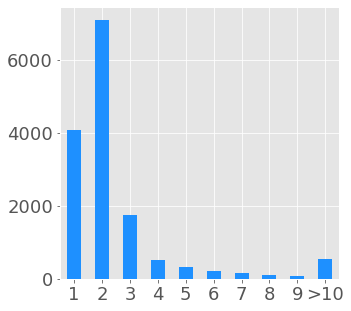
\includegraphics[width=\textwidth]{images/hist_amount_of_people.png}
         \caption{Histogram of amount of people detected by AlphaPose.}
         \label{subfig:amount_of_people_hist}
     \end{subfigure}
     \hfill
     \begin{subfigure}[b]{0.4\textwidth}
         \centering
         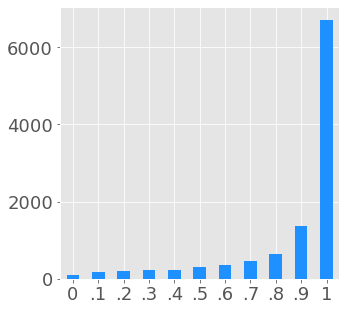
\includegraphics[width=\textwidth]{images/hist_signers_scores.png}
         \caption{Histogram of signer-confidence scores (rounded to one decimal).}
         \label{subfig:signers_scores_hist}
     \end{subfigure}
    \caption{Amount of signers and signer scores histograms.}
    \label{fig:signers_statistics}
\end{figure}

To infer the signer, we first obtained the keypoints and bounding boxes of the people in each video. This was done using AlphaPose with the Halpe full-body keypoints format \cite{fang2017rmpe}. This format has 136 keypoints of which 42 are hand keypoints, which makes them suitable for hand gesture recognition. Then, we transformed each keypoints' coordinates to a relative position with respect to the person's center. For each person in the video, we computed the total amount of movement of their hands. The person chosen as the signer is the one who has the largest amount of hand movement, with a high confidence (Figure \ref{subfig:signers_scores_hist}). 

The resulting keypoints computed by AlphaPose, the result of the signer inference and the amount of movement of each person used to compute the confidence score of the inference are provided for each sample of the dataset.


% in a pair of consecutive frames as the sum of the euclidean distance between both of its hands' keypoints position in one frame to the position in the next one. The total movement of the video is then the sum of the hands movements for each pair of consecutive frames in the video. Finally, 
 

%We also propose a score that reflects how confident is the signer choice: for a video with \(|S|\) signers and being \(max_1(S)\) and \(max_2(S)\) the highest and second-highest movement amount of the signers respectively, the score is computed as \(\frac{max_1(S) - max_2(S)}{max_1(S)}\). Figure \ref{subfig:signers_scores_hist} shows an histogram of the scores for all samples. It can be seen that most of the computed scores are between 0.9 and 1 (\(\sim 75\%\)), so it could be considered safe to dismiss videos with lower scores when training a model without losing an important number of samples.

% Also, for a video with \(|S|\) signers and being \(max_1(S)\) and \(max_2(S)\) the highest and second-highest movement amount of the signers respectively, a score that reflects how confident is the signer choice is computed as \(signer\_confidence(S) = \frac{max_1(S) - max_2(S)}{max_1(S)}\). So \(signer\_confidence(S)\) represents the difference between the movement of the person chosen as the signer and the second most probable one normalized by the movement of the chosen signer. Then, \(signer\_confidence(S) = 0\) means that the chosen signer and the second option had the same amount of movement, while \(signer\_confidence(S) = 1\) means the second most probable person to choose as the signer did not move at all. Figure \ref{subfig:signers_scores_hist} shows an histogram of the scores (rounded to two decimals) for all samples and it can be seen that most of the computed scores are between 0.9 and 1 (\(\sim 75\%\)), so it could be considered safe to dismiss videos with lower scores when training a model without losing an important number of samples.

